\documentclass[11pt]{article}
\usepackage{cite}
\usepackage[useregional]{datetime2}
\usepackage{babel}
\usepackage{graphicx}

\usepackage{multirow}
\usepackage{dirtytalk}
\usepackage{geometry}
\geometry{
    a4paper,
    total={170mm,257mm},
    left=20mm,
    %right=40mm,
    top=20mm,
    marginparsep=-7mm,
    marginparwidth=20mm
}


\usepackage{setspace}
\doublespacing

% shrink marginpar font size
\let\oldmarginpar\marginpar
\renewcommand\marginpar[1]{\-\oldmarginpar[\raggedleft\footnotesize #1]%
{\raggedright\footnotesize #1}}

\begin{document}

\title{Understanding and Avoiding AI Failures: A Practical Guide}
\author{Max Williams \\ University of Louisville \and Roman Yampolskiy \\ University of Louisville}
\date{\today}
\maketitle
\newpage

\tableofcontents
\newpage

%\listoffigures
%\newpage
%\listoftables
%\newpage

\abstract{
    In place of root cause analysis, we look over the history of accidents involving AI to find
    common themes between these failures to develop a rudimentary guide as to what failures to
    expect based on the nature of a technology and means to mitigate the damage or a recommendation
    to unilaterally discontinue research in extreme cases. By focusing on systems analysis instead
    of root cause, we can systematically identify when and where attention should be paid to safety
    of current generation AI systems.}
\newpage

\newpage
\section{Introduction}
\label{sec:introduction}

With current AI technologies, harm done by AIs is limited to power that we directly put in their
hands.  As said in \cite{yam2018historic}, ``For Narrow AIs, safety failures are at the same level
of importance as in general cybersecurity, but for AGI it is fundamentally different.'' Despite AGI
still being well out of reach, the nature of AI catastrophes has already changed in the past two
decades. Automated systems are now not only malfunctioning in isolation, they are interacting with
humans and with each other in real time. This shift has made traditional systems analysis more
difficult, as the other entities interacting with any given AI are neither homogeneous nor rational.

In response to this, we analyze how risks associated with complex control systems has been managed
historically and contemporary AI failures to create a framework for predicting what kinds of risk
are created from the operation of any AI system. We create a framework for analyzing AI systems
before they fail to understand how they change the risk landscape of the systems they are embedded
in, based on conventional system analysis and open systems theory as well as AI safety principles.

\newpage
\section{Terminology}

\begin{itemize}
\item Systems accident: An accident in a system with high complexity and tight coupling caused by complex
interactions between system components. They are often incomprehensible to operators.
\cite{perrow1999living}

\item Normal accident: Synonym for Systems Accident. ``Normal" here refers to the inevitability of the
accident from the system's functioning often despite best efforts to avoid an accident.

\item Tight coupling: Two components are tightly coupled if one depends on the other, especially if this
dependence happens on a very short time scale.

\item Loose coupling: Two components are loosely coupled if one depends on the other indirectly or if there
is a lot of time in the interaction

\item Slack: Redundancy and time for errors to be noticed both create slack. Highly redundant systems are
often designed with lots of slack, which is used up as components degrade over time or under
stress. Slack also refers to the divergence of metal models used by operators, creating mental
redundancy that makes it more likely that a problem is solved correctly. [TODO make sure I'm
understanding slack correctly here and elsewhere]
\end{itemize}

\marginpar{Is a bulleted list okay here?}

\newpage
\section{Related Work}

\subsection{Early History}

As computer control systems increased in complexity in the 70's and 80's, unexpected and sometimes
catastrophic behaviour would emerge from previously stable systems \cite{anderson2005control}. While
linear control systems had been used for some time (for example, a thermostat) without unexpected
behaviour, adaptive control systems created novel and unexpected problems, such as ``bursting''. As
described in \cite{anderson2005control}, bursting is the phenomenon where a stable controller would
function as expected for a long time before bursting into oscillation, then returning to a stable
state. This is caused by the adaptive controller not having a rich enough input during the stable
period to determine the unknown coefficients of its model correctly, causing the coefficients to
drift. Once the system enters oscillation, the signal again becomes rich enough for the controller
to correctly estimate the unknown coefficients and the system becomes stable again. The increased
complexity of the more advanced technology (dynamic controller instead of a  static controller)
introduced a dynamic not present in previous technologies, and incomprehensible to an operator not
familiar with this behavior. Worse, since this behavior only happens when the controller is
controlling the real world plant, designers had no way of predicting this failure mode. Bursting can
be reduced using specifically engineered safety measures or more complex controllers (which bring
even harder to understand problems), but still demonstrates that increases in complexity always
bring risk.

\subsection{Normal Accident Theory}

Risk of failure is a property inherent to complex systems, and complex systems are inherently
hazardous \cite{cook1998complex}.  At a large enough scale, any system will produce ``Normal
Accidents''. These are unavoidable accidents caused by a combination of complexity, coupling between
components, and potential harm. A normal accident is different from the more common component
failure accidents in that the events and interactions leading to normal accident are not
comprehensible to the operators of the system \cite{perrow1984living}. Increasing the complexity
and broadening the role of AI components in a system decreases comprehensibility of the system,
leading to an increase in normal accidents.

In 1984, Charles Perrow published ``Normal Accidents" \cite{perrow1984living} which laid the
groundwork for NAT (Normal Accident Theory). Under NAT, any system that is tightly coupled
and complexly interactive will inevitably experience a systems accident. Decentralization reduces
coupling and increases complexity, while centralization decreases complexity but also increases
coupling. Thus, since an organization cannot be both centralized and decentralized, large
organizations will harbor system properties that make them prone to normal accidents.

\subsection{High Reliability Theory}

% quote of the day: One of the principal values of `normal accident' analysis and case descriptions
% is that it helps to develop convincing materials to counter the naive, perhaps wistful or
% short-sighted, views of decision-makers who, due to institutional  pressure, desperation or
% arrogance, are temped to make unrealistic assumptions about the systems they direct but for which
% they have only nominal operational responsibility. 
% https://onlinelibrary.wiley.com/doi/10.1111/j.1468-5973.1994.tb00045.x

High reliability theory was developed to explain the incredible ability of certain organizations to
function without major accidents for long periods of time. In \cite{weick1999reliability}, Weick
identifies several common traits shared by high reliability organizations (HROs): a strategic
prioritization of safety, careful attention to design and procedures, a limited degree of
trial-and-error learning, redundancy, decentralized decision making, continuous training often
through simulation, and strong cultures that encourage vigilance and responsiveness to potential
accidents.  

% This is off topic but it struck me as important so I'm leaving it in for now
High reliability organizations manage the apparent paradox proposed in normal accident theory by
having traits of both centralization and decentralization. Decision making is decentralized,
allowing for decoupling while policy and cultural factors are highly centralized, allowing for the
unification of goals and attention to safety. This ability to be simultaneously centralized and
decentralized through common culture and goals is present not only in HROs but many post-industrial
societies as identified by Hofstadter in [TODO cite, or maybe delete this paragraph as being
off-topic]

\subsection{NAT-HRT Reconciliation}

Normal accident theory holds that for certain kinds of industries systems accidents are inevitable.
Meanwhile, high reliability theory makes the observation that there are many exceptions to this, and
there are common traits shared by these ``high reliability organizations" (HROs) that can be studied
and understood as indicators of reliability. In \cite{shrivastava2009normal}, Shrivastava et al
analyze works which frame these two theories as being in conflict then reconcile the two theories.

Normal accident theory states that a system has to choose to trade off between centralization (which
allows for organization-aligned action and less chaos) and decentralization (which allows and
enables operators to quickly make decision). High reliability theory considers that it is possible
to escape this apparent paradox by allowing operators a high level of autonomy (decentralized
decision making) while also putting a focus on cultural aspects that improve safety and reliability
(centralized goals).

Shrivastava et al use the Swiss cheese model (SCM) to explain the importance of time in the
occurrence of accidents, even in systems that are stable over time. In the SCM, the layers of safety
are modeled as slices of cheese with holes in them representing weak points in each layer of safety.
Over time, holes change shape and move around. Eventually, no matter how many slices of cheese
(layers of safety) there are, the holes will align allowing a straight shot through all of the
slices of cheese (an accident occurs) [TODO cite Reason, 1998]. However, the SCM model only helps
understand that accidents are inevitable, and ``inevitability is immaterial for practical purposes"
as Shrivastava et al state, since the time scales involved for some systems may be too great to
consider possible.

Disaster incubation theory (DIT) is also introduced as the final piece needed to reconcile normal
accident theory and high reliability theory. DIT describes how organizations gradually migrate to
the boundary of acceptable behavior, as good safety records drive up complacency and deviance is
normalized [TODO cite Vaughan 2005, Rasmussen, 1997]. DIT was considered only useful in hindsight by
proponents of NAT, so Snook [TODO cite Snook 2000] investigated accidents with this in mind and
created the framing of ``practical drift". This is the `slow steady uncoupling of local practice
from written procedure' which leads an initially highly coupled system to become uncoupled from
operators and managers optimize their processes to be more efficient, deviating from procedure.
Then, if the system is required to become tightly coupled again, the operators are ill-prepared for
this increase in coupling and systems accidents become far more likely.

\marginpar{these paragraphs are a bit hard to read and boring}

Through the lens of disaster incubation theory and practical drift, Shrivastava et al explain how
NAT and HRT actually work to compliment each other to explain how accidents take place and are
avoided. The time period being considered by HRT takes place while the system is still a high
reliability organization. The culture and procedures put in place are working correctly, coupling is
high and complexity is manageable to the well trained operators. Over time, however, practical drift
decouples the system, and reliability decreases. If the organization is a high reliability
organization, degradation is limited and incidents can still be managed. Accidents that take place
during this period of time are within the scope of HRT. However, there is the possibility for an
unlikely event to lead from this steady decline of reliability into the normal accident of NAT. If
the system suddenly has to become more coupled (for instance, during a special mission or to react
to an incident breaking down multiple layers of safety mechanisms), it is ill prepared to do so. At
this point, NAT's trade-off between coupling and complexity becomes important, and the perceived
complexity of the system increases drastically, making safe operation impossible, leading to a
normal accident. This can only happen after a great decrease in coupling from the initial (designed)
state of the system, so proponents of HRT would say that the accident was only able to take place
due to the system no longer acting as a high reliability organization. 

Thus high reliability theory can serve to understand how organizations resist practical drift, and
the accidents that happen when practical drift leads to accidents. Normal accident theory is useful
when practical drift has lead to a great degree of decoupling, then a sudden change in situation
(which may be an intentional operation or an incident) leads to the need to increase coupling, which
the system is (surprisingly, to operators) no longer able to handle without increasing complexity
beyond manageable levels. 

\subsection{Lethal Autonomous Weaponry}

The introduction of lethal autonomous weaponry \cite{carvin2017normal} increases the danger of
normal accidents not because it provides new kinds of failure or novel control system but because of
the drastically increased potential harm. A machine which kills when functioning
correctly is much more dangerous in an accident than one which only does harm when malfunctioning.
By increasing the level of complexity and autonomy of weapons systems, normal accidents involving
powerful weapons becomes a possibility.

\subsection{Robustness Issues for Learned Agents}

In \cite{uesato2018adversarial}, Jonathan Uesato et al show that by training a reinforcement learner
in an environment with adversarial perturbations instead of random perturbations, failure modes that
would be extremely unlikely to be encountered otherwise were detected and integrated into training.
This shows that AI trained to be ``robust'' by training in a noisy environment may have catastrophic
failure modes that are not observed during training but can spontaneously occur after deployment in
the real world. Adversarial training is a tool to uncover and improve these issues, but is only an
engineering safety measure over the deeper issue of black box AI which are not characterized of
their entire input space.

\subsection{Examples of AI Failures}

Large collections of AI failures and systems to categorize them have been created before
\cite{yam2018historic} \cite{scott2020classification}. In \cite{scott2020classification}, the
classification schema details failures by problem source (such as design flaws, misuse, equipment
malfunction, etc.), consequences (physical, mental, emotional, financial, social, or
cultural), scale of consequences (individual, corporation, or community), and agency (accidental,
negligent, innocuous, or malicious). It also includes preventability and software development
life-cycle stage.

\subsection{Societal Impact of AI}

The proliferation of AI technologies has impacts in our socioeconomic systems and environment in
complicated ways, both positive and negative \cite{jayden2018sustainability}. AI has the ability to
make life better for everyone but also to negatively impact many by displacing workers and
increasing wealth disparity [TODO find a citation that isn't a news source]. This is just one
example of AI interacting with a complicated system (in this case, the job market) to have large
scale consequences. 

\subsection{AI Safety}

The field of AI safety focuses on long-term risks associated with the creation of AGI. The landmark
paper ``Concrete Problems in AI Safety" \cite{amodei2016concrete} identifies the following problems
with current and future AI: avoiding negative side effects, avoiding reward hacking, scalable
oversight, safe exploration, and robustness to distributional change. Other topics identified as
requiring research priority by other authors include containment \cite{james2016containment},
high reliability, error tolerance, value specification \cite{soares2017foundations}
\cite{hadfieldmenell2020inverse}, and superintelligence \cite{bostrom2001extinction}
\cite{bostrum2014superintelligence}. These topics are all closely related, and could all be
considered an instance of the ``Do What I Mean" directive \cite{yudkowsky2011dwim}. We will explore
the five topics form \cite{amodei2016concrete} with examples of failures and preventative measures
where applicable. 

\subsubsection{Avoiding Negative Side Effects}

This problem has to do with things that are done by accident or by indifference by the AI. A
cleaning robot knocking over a vase is one example, and complex environments have so many kinds of
``vases" that we are unlikely to be able to program in a penalty for all side effects
\cite{amodei2016concrete}. One of the AI Safety Gridworlds features a task of moving from one
location to another without putting the environment in an irreversible state
\cite{leike2017gridworlds}. To be able to avoid negative side effects, an agent has to understand
the value of everything in its environment in relation to the importance of its objective, even
things that the reward function is implicitly indifferent towards. Knocking over a vase is acceptable
when trying to save someone's life, for example, but knocking over a building is less so. Many
ethical dilemmas encountered by people are concerned with weighing the importance of various side
effects, such as environmental pollution from industrial activity and animal suffering from farming,
so in general this is a non-trivial problem even for humans. However, using ``common sense" to avoid
damaging the environment while carrying out ordinary tasks is a realistic and practical goal with
our current AI technologies. Inverse reward design, which treats the given reward function as
incomplete, is able to avoid negative side effects to some degree \cite{hadfieldmenell2020inverse}.

\subsubsection{Avoiding Reward Hacking}

Most AI systems designed today contain some form of reward function that should be optimized. Unless
designed with safety measures to prevent reward hacking, the AI can find ways to increase the reward
signal which don't complete the objective. These might be benign, such as using a bug in the program
to set the reward to its highest value [TODO cite?], complicated such as learning to fall over
instead of learning to walk \cite{lehman2018surprising}, or dangerous, such as coercing human
engineers to increase its reward signal by threatening violence.

Agents that wish to hack their rewards can do so by breaking out of their containers, whether they
are simple training environments or carefully engineered prisons with defenses in depth
\cite{james2016containment}.  When researching novel AI that has a risk of becoming AGI, researchers
must use safety measures to prevent the AGI from escaping confinement. This is currently not a
common practice as AI today are not believed to be capable of escaping the simulations they are
tested in. However, humans and AI have both broken confinement in games that are used to benchmark
AI. In 2018, an AI designed to maximize the score in a video game instead performed a series of
seemingly random actions which caused the score to increase rapidly without continuing to progress
in the game \cite{chrabaszcz2018qbert}. In this example, the AI is supposed to be using the game
controller output to move the character around the screen to play the game and maximize the score,
but it instead learned to hack the game and obtain a much higher score than is conventionally
possible.  Through an exploit in the game's programming, the AI managed to directly modify its score
instead of taking actions within the simulation as expected. In 2014, an exploit in Super Mario
World was used to modify memory and jump directly to the end screen of the game a few minutes into
play. This also demonstrates an agent (in this case, computer assisted human) breaking a level of
containment through a sophisticated attack.

In light of these examples, it is possible to gain arbitrary code execution abilities from within a
sandboxed game environment, and these kinds of exploits may be present inside any program which is
meant to limit the output space of an AI. Virtual machines, often used as an additional layer, as
also susceptible to a wide range of exploits \cite{reuben2007virtual}.  This illustrates a more
general concern which is the AI acting outside of the output space that it was designed to work
with, seen in many of the AI failures in \cite{yam2018historic}.

Adversarial reward functions, where the reward function is learned and has a completing objective
with the AI, can decrease reward hacking \cite{fu2018adversarial}. To detect reward hacking,
tripwires can be used. For instance, if the AI gets a much higher score than expected to be possible 
then it can be assumed that it has broken containment and is modifying the reward directly.

\subsubsection{Scalable Oversight}

Designers have only so much resources to monitor the actions of the AI. External factors are
inevitably forgotten about (worsening side effects) and reward functions fail to perfectly
capture what we really want (worsening reward hacking).
,....

\subsubsection{Safe Exploration}

....


\newpage
\section{Classification Schema for AI Systems}
\label{sec:classification}

We present a tag based schema similar to the one presented in \cite{scott2020classification}.
Instead of focusing on AI failures, this schema classifies the AI and the system the AI is embedded
in, allowing for risk analysis prior to failure. We pay
particular attention to the orientation of the AI as both a system with its own inherent dangers
and a as component in a larger system which depends on the AI. Any
analysis attempting to divide a system into components must acknowledge the `ambiguities, since once
could argue interminably over the dividing line between part, unit, and subsystem'
\cite{perrow1984living}. The particular choice of where to draw the line between the AI, the system,
and the environment are important to making a meaningful analysis, and requires some intuition.
Because of this, out classification system encourages repeating parts of it for different choices of
dividing lines between AI and system to encourage finding the right framing.

To characterize the risk of an AI system, one factor is the dangers expressed by the
larger system in which the AI is a component. In an experimental setting, a genetic algorithm
hacking the simulator can be an amusing bug \cite{lehman2018surprising}, but a similar bug making
its way into an autonomous vehicle or industrial control system would be potentially
dangerous. Understanding the risks involved in operating the system which the AI belongs to is
critical in understanding the risk from this particular AI application.

The AIs outputs must be connected to some means of control to be useful within the system. This can
take many forms: indirectly, with AI informing humans who then make decisions, or directly with an
AI controlling the actuators of a robot or chemical plant. Any production AI system has some degree
of control over the world, and it may not be clear where the effects of the AI take place. This
connection, where the output of a component (the AI) has significant effects on other components or
system properties is an instance of coupling. Because there are multiple components affected by the
AI and those components are themselves coupled with other components, we frame this problem in terms
of the AI and a `target' which the AI can affect.  For example, the output from an AI meant to
control the flow speed of a valve in a chemical plant can be framed in numerous ways: the software
signal with the computer the AI is running in, the electrical output from the controller, the
actuation of valve, the rate of fluid flowing through the valve, or a variable in the chemical
reaction taking place downstream. Understanding what the target of the AI is depends on context, and
all of these targets have unique consequences the might be overlooked in analyzing just one of them.
The classification schema allows for as many targets as needed when analyzing a system.

Observability of the warning signs of an accident is important as it allows for interventions by
human operators, a crucial tool in preventing accidents (``People continuously create safety''
\cite{cook1998complex}). The likelihood of timely human interventions depends on four things:
\begin{itemize}
    \item Time delays between AI outputs and the effects of the target.
    \item Observability of the system state as it is relevant to potential accidents.
    \item Frequency and attention paid by human operators.
    \item Ability of operators to correct the problem once it's been identified.
\end{itemize}


The time delay between an AI creating an output and that output affecting the target is essential to
preventing accidents.  Tightly coupled systems with short time delays (such as automated stock
trading) are more hazardous because the system can go from apparent normalcy to catastrophe faster
than operators can realize there is something wrong \cite{andrei2017flash}.
Observability and attention from human operators are needed for these time delays to be an effective
component of safety. As the level of automation of a system increases, human operators become less
attentive and their understanding of its behavior decreases \cite{bainbridge1983ironies}. Reliance
on automated systems decreases an operator's ability to regain control over a system if an accident
requires manual control. For example, if an autonomous driving system fails, the driver, now less
familiar with driving, has to suddenly be in manual control. Together, observability, human
attention, and human ability to correct possible failures in the system all make up a major factor
in whether or not a malfunction leads to an accident.

For a given choice of target being controlled by the AI, there is maximum conceivable amount of
damage that can be done by malicious use of that target. We use the figure as a cap as to the amount
of harm possible. Most AI failures are not malicious [TODO cite, maybe?], so the harm done by an
accident will almost always be much less than this amount. This factor is very difficult to predict
prior to an accident. For example, imagine a component which controls cooling for a nuclear plant.
One could say the maximum damage from its malfunctioning is a lost day of productivity because of
the backup cooling system. Another might say loss of the entire core is possible if the backup
system also malfunctions, but the containment system is sure to keep it from harming anyone outside.
Yet another might notice that containment could also fail, and a meltdown could harm millions of
people in surrounding towns. Because of the unpredictability of how much harm one system could do,
this factor is included as a rough estimate of the scale of power the AI has over the system and the
system has over the environment. 

The final criteria for classifying the nature and degree of systems risk of an AI system are
coupling, complexity of interaction, energy level, and knowledge gap. Coupling is a measure of the
AI's interconnectivity with other components in the system, and the strength of these connections.
Loosely coupled systems have sparse connectivity which limits the propagations of component failure
into an accident, but are also less robust. Tightly coupled systems have dense connectivity and many
paths between components, and often feedback loops that allow a component to affect itself in
complicated ways \cite{perrow1984living}. Classifying the level of coupling of the system in
proximity to the AI component can be difficult and nebulous, so only course categories (loose,
medium, tight) are used in this analysis as finer grained considerations are likely to become
arbitrary.

Coupling considers other components and aspects of the environment that the AI is coupled with.
Examples of coupling include taking data in from another component, transmitting data to another
component, relying on the functioning of a component, having another component rely on the
functioning of the AI, an aspect of the environment the AI directly or indirectly affects by its
decisions. For each coupled component, score on a scale of 1-5 from loosely coupled to strongly
coupled, and sum these scores to get the total degree of coupling.

Complexity of interaction is a measure of how complex these interactions are. Linear interactions
are simple to understand and behavior is easy to extrapolate from a few observations. Complex
interactions have sudden non-linearities and bifurcations [TODO this paragraph has a lot of potential
but I'm not ready to write it yet].

Energy level is the amount of energy available to or produced by the system. Low energy systems are
systems such are battery operated devices, household appliances, and computers. Medium energy
systems include transportation systems, small factories, and mining. High energy systems include
space travel, nuclear power and some chemical plants.

Knowledge gap is the gap between how well technology is understood and the scale of its use.
Technologies very early in the technological readiness scale [TODO cite] have a large knowledge gap
if used in production systems. Likewise, technologies that are very well developed and understood
can be used in production without creating a knowledge gap, so long as appropriately trained
personnel are operating them. [TODO more here]

Analysis done in the field of AI safety frequently addresses dangers associated with artificial
general intelligence (AGI) and superhuman intelligence. In Section \ref{sec:introduction} we gave an
cursory overview of the dangers of AGI. Certain classes of contemporary AI exbibit some of the
dangers that true AGI could manifest, thus considerations such as containment and reward hacking are
useful in analyzing AI applications, even if the existential threat of AGI isn't present.  We also
include a risk factor for research which may lead to the development of AGI in our analysis. These
dangers will be referred to as ``AI safety" [TODO is this a good name?] which are treated from an AI
safety perspective as opposed to the other safety considerations which we consider ``system safety"
[TODO also this name isn't great].

\begin{figure}[h]
    \centering
    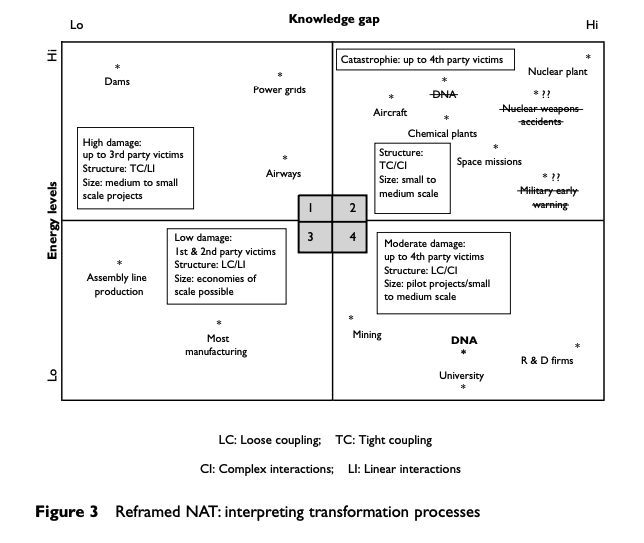
\includegraphics[width=0.6\textwidth]{images/reframed-nat-2axis}
    \caption{[TODO this needs to be mentioned in the text] Plotting energy level against knowledge
    gap to create 4 quadrants, from \cite{shrivastava2009normal}}
    \label{fig:quad}
\end{figure}

The following factors are considered most significant to understanding the level and nature of
the risk of a system utilizing AI:

\begin{itemize}
    \item The system which is affected by the outputs of the AI
    \item Time delay between AI outputs and the larger system, system observability, level of human
        attention, and ability of operators to correct for malfunctioning of the AI
    \item The maximum damage possible by malicious use of the systems the AI controls
    \item Coupling of the components in proximity to the AI and complexity of interactions
    \item Knowledge gap of AI and other technologies used and the energy level of the system
\end{itemize}

\subsection{Time Delay, Observability, Human Attention, and Correctability}

A rough time span should be given to indicate how long it takes for the AI component in
consideration to have a significant effect on the target in question. Only an order of magnitude
(``minutes" vs. ``hours" vs. ``days") is needed.

Observability measures how observable the internal state of the system is, how often and with what
degree of attention a human will attend to the system, and how easy or difficult a failure of the AI
component of the system is to correct once detected.

Observability is measured on a scale of 0-5, from 0 for a complete black box to 5 for AI whose
relevant inner workings can be understood at a glance.

Human Attention is measured as the number of hours in a day that an operator will spend monitoring
or investigating the AI component when there have not been any signs of malfunction. If the system
is not monitored regularly, then this is instead written as the amount of time that will pass
between checkups.

\subsection{Target of AI Control}

All steps with an asterisk (*) should be repeated for each possible target. Targets should be chosen from a
wide variety of scales for the best analysis.

\subsection{Single Component Maximum Possible Damage*}

This is the amount of damage that could be done by a worse case malfunctioning of the AI component
by itself. Since the actual worse case would be unimaginably unlikely or require superhuman AI in
control of the AI component, we instead approximate the expected worse case by imagining a human
adversary gaining control of the AI component and attempting to do as much harm as possible. This
should consider both monetary damage, harm to people, and any other kinds of harm that could come
about in this situation.

\subsection{Coupling and complexity*}

Together, coupling and complexity are used to asses the risk of experiencing a systems accident.
Use Table \ref{tab:nat} to convert coupling (high, medium, low) and interaction complexity
(linear, moderate, complex) to find the risk of a systems accident (\underline{L}ow,
\underline{M}edium, \underline{H}igh, \underline{C}atastrophic).

\begin{table}[h]
\centering
\begin{tabular}{|l|l|l|l|}
\hline
\multirow{2}{*}{Coupling} & \multicolumn{3}{l|}{Interaction} \\ \cline{2-4}
        & Linear & Moderate & Complex \\ \hline
High    & M      & H        & C       \\ \hline
Medium  & L      & M        & H       \\ \hline
Low     & L      & L        & M       \\ \hline
\end{tabular}
\caption{Using coupling and interaction level to determine the severity of accident the system may
    experience. Adapted from \cite{shrivastava2009normal}.}
\label{tab:nat}
\end{table}

\subsection{Energy Level and Knowledge Gap*}

Energy level and knowledge gap are used together to predict the potential damage from a system
accident and the parties involved in such an accident using Table \ref{tab:nat2}. The first letter
is the amount of damage (\underline{L}ow, \underline{M}edium, \underline{H}igh) and the number is
the degree of separation between the system and the potential victims of the accident. First-party
victims are operators, second-party victims are non-operating personnel and system users, third
party victims are unrelated bystanders, fourth party victims are people in future generations
\cite{shrivastava2009normal} [TODO they attributes this to ``accident literature", but citing a
concrete source would be better].

\begin{table}[h]
\centering
\begin{tabular}{|l|l|l|l|}
\hline
\multirow{2}{*}{Energy Level} & \multicolumn{3}{l|}{Knowledge Gap} \\ \cline{2-4}
     & Low & Med & High \\ \hline
High & H3  & H3  & C4   \\ \hline
Med  & M3  & M3  & H4   \\ \hline
Low  & L2  & L2  & M4   \\ \hline
\end{tabular}
\caption{Using energy level and knowledge gap to determine amount of damage (Low, Medium, High,
Catastrophic) and distance to potential victims (1st party, 2nd party, 3rd party, 4th party).
Adapted from \cite{shrivastava2009normal}.}
\label{tab:nat2}
\end{table}

\section{AI Safety Evaluation}
\label{sec:aisafety}

In this section, we evaluate AI safety concerns, without being concerned about the details of the
system the AI is being used in. While no current AI systems pose an existential threat, the
possibility of a ``foom" scenario \cite{bostrom2001extinction} is considered seriously as it is
unknown how far we are from this points, and recent advancements (such at GPT-3
\cite{brown2020gpt3}) remind us how rapidly AI capabilities can increase. In this section we
create a schema for classifying the AI itself in terms of autonomy, oversight, and escape potential.

\subsection{Autonomy}

While autonomy is hard to pin down, we all know how to identify it. Or as Supreme Court justice
Potter Stewart said, ``I'll know it when I see it". [TODO this sentence is a joke, remove it and
probably this subsection]

Level 0: Little or no autonomy, the program is explicitly designed and won't act in unexpected ways
except due to bugs, and this unexpected behavior is unintelligent in nature.

Level 1: An optimization process is used, but not one that will attempt to break out of confinement.
Examples of this include gradient descent and other standard machine learning algorithms. Image
classifiers and GPT-3 are expected to be in this class, although there is speculation that with some
prompts GPT-3 could emulate enough of a dangerous mind to attempt a break at confinement. 

Level 2: The program is designed to have agency, and interacts with the environment (even a
simulated one) in a goal-directed way. The includes reinforcement learners and agents learned by
genetic algorithms

Level 3 (danger): A practical understanding of self, and theory of other minds develops

\subsection{Goal Observability}

Software that has very simple functionality (such as a thermostat) has completely comprehensible
goals, to the extent that we hardly consider them goals so much as the system's only functionality.
More complex software may use an optimization process to maximize some objective function (or
minimize a loss function), which provides a goal which is understandable, but the goal seeking
behavior of the agent may not be. 

\begin{itemize}
\item Level 0: Programs that ``just run" and have no goal seeking behavior 
\item Level 1: Basic goal seeking behavior such as numerical optimization
\item Level 2: Complex goal seeking with the ability to seek subgoals and express reward hacking
\item Level 3 (danger): Ability to realize instrumental goals and seek self improvement
\end{itemize}

\subsection{Escape Potential}

\begin{itemize}
\item Level 0: None
\item Level 1: The agent may find unexpected behaviors which technically achieve the goal but are not desirable
\item Level 2: The agent intentionally seeks to hack its environment
\item Level 3 (danger): The agent has the ability and drive to break through most cybersecurity and
                        containment procedures 
\end{itemize}

\subsection{Anthropomorphization}

\begin{itemize}
\item Level 0: Obviously a machine
\item Level 1: Some surface level appearance of humanity (natural language interaction, robot
        chassis with human features, a name and supposed personality) 
\item Level 2: Level 1 but with software to support the illusion of humanity (speech interaction,
        human-ish actuated movements) 
\item Level 3 (danger): The AI can be mistaken for a human even with unrestricted communication (may be
        text-only, voice, or in person) 
\end{itemize}

\newpage
\section{Determining Risk Using Schema Tags}
\label{sec:determining}

The following tables use scheme tags developed in Section \ref{sec:classification} can be used for
determining the next steps in risk assessment.


\begin{center}
\begin{tabular}{ |l|l| } 
 \hline
 Time Delay & (seconds, minutes, hours, etc.) \\
 \hline
 Observability & 0-5\\
 \hline
 Human Attention & (N times per day OR intermittent, (days, weeks, months)) \\
 \hline
 Correctability & 0-5 \\
 \hline
\end{tabular}
\end{center}

\begin{center}
\begin{tabular}{ |l|l|l|l| } 
 \hline
 Targets & max damage & system accident risk & potential damage to other parties\\
 \hline
 Target 1 & \$n & (L, M, H) & (L, M, H, C) (1, 2, 3, 4) \\
 ...      &     &           &                           \\
 Target n & \$n & (L, M, H) & (L, M, H, C) (1, 2, 3, 4) \\
 \hline
\end{tabular}
\end{center}


\newpage
\section{Case Studies}

We will analyze systems that use AI in the present, historically, and from fiction under this
framework, and provide analysis of where their risk lies and what measures are recommended in those
situations.

Posthumous analysis of accidents makes it very easy to point fingers at dangerous designs and
failure by operators. However, safety is very difficult, and often well-intentioned attempts to
increase safety can often make accidents more likely either by increasing coupling and thus
complexity, or increasing centralization and thus brittleness \cite{perrow1999living}. Because of
this, we will not be attempting to use hindsight to prevent accidents that have already happened.
Instead we will be focusing on systems which have yet to fail but might at some point.

\subsection{Roomba House Cleaning Robots}

AI component: VSLAM mapping and navigation algorithm

\subsubsection*{Time Delay}

There is minimal delay between navigation and robot movement, likely milliseconds or seconds.

\subsubsection*{System Observability}

While operating, it is not possible to tell where the Roomba will go next,
where it believes it is, or where it has been unless the user is very familiar with how it works in
the context of their floor plan. Some models include software for monitoring the robot's internal
map of the house, but it is not likely to be checked unless something has gone wrong. However, it is
very simple to correct, as the robot can be factory reset.

\subsubsection*{Human Attention}

The user is unlikely to notice the operations of the robot except if something goes wrong. If the
robot is not cleaning properly or has gone missing, the user will likely notice only after the
problem has emerged.

\subsubsection*{Correctability}

Since the robot is replaceable and manual cleaning is also an option if the robot is out of order,
correcting for any failure of the robot is simple.

\subsubsection*{System Targets} 

\begin{enumerate} 
\item Movement of the robot within a person's home
\item Control over which areas of the floor have or have not been vacuumed
\end{enumerate}

\subsubsection*{Maximum damage by malicious use}

\begin{enumerate}
\item Household environment: Average of a few hundred dollars per robot. Given full control of
the Roomba's navigation, a malicious agent may succeed in knocking over some furniture, and could
also be able to destroy the Roomba by driving it down stairs or into water. And the house would not
be cleaned (denial of service).
\item Floor Cleanliness: Possible inconvenience if the floor is left dirty.
\end{enumerate}

\subsubsection*{Coupling}

\begin{enumerate}
\item Household environment: The robot is moderately coupled with the environment it is in, because
it is constantly sensing and mapping it. Small changes to the environment may drastically change its
path. 
\item Floor Cleanliness: The cleanliness of the floor is coupled to the robot, failure of the robot
will result in the floor being unexpectedly dirty. However, this happens over a slower time frame so
it is only loosely coupled.
\end{enumerate}

\subsubsection*{Complexity}

\begin{enumerate}
\item Household environment: Moderate complexity, the user may not understand the path the robot
takes or how it can become trapped, but the consequences for this are minimal.
\item Floor Cleanliness: Linear, the robot works and makes the floor clean or it doesn't and the
floor slowly gets dirty over time.
\end{enumerate}

\subsubsection*{Energy Level}

The robot runs off a builtin battery and charges from a wall outlet. It is well withing the `Low'
level of energy as a household appliance.

\begin{enumerate}
\item Household environment: Low
\item Floor Cleanliness: Low
\end{enumerate}

\subsubsection*{Knowledge Gap}

There is minimal disparity between design and marketing, as the software was designed in-house. Some
unexpected aspects of the environment may interact poorly with it (for example, very small pets that
could be killed by the robot). The other technologies (vacuum cleaners, wheeled chassis robots) are
also very mature and well understood, so there is no knowledge gap for any other components. This
puts it in the `Low' category for knowledge gap.

\begin{enumerate}
\item Household environment: Low
\item Floor Cleanliness: Low
\end{enumerate}


\subsubsection{Tabular format}

\begin{center}
\begin{tabular}{ |l|l| } 
 \hline
 Time Delay & seconds \\
 \hline
 Observability & 3 \\
 \hline
 Human Attention & intermittent, weeks \\
 \hline
 Correctability & 5 \\
 \hline
\end{tabular}
\end{center}

\begin{center}
\begin{tabular}{ |l|l|l|l| } 
 \hline
 Targets & max damage & system accident risk & potential damage to other parties\\
 \hline
 Robot movement & \$200 & M & L2 \\
 Cleanliness of floor & \$0 & L & L2 \\
 \hline
\end{tabular}
\end{center}

\subsubsection{AI Safety Concerns}

The system is level 0 in all categories in Section \ref{sec:aisafety}. This placers it within the
category of weak AI and presents no possibility for unbounded improvement or unfriendly goal seeking
behavior.

\subsubsection{Suggested Measures}

[TODO this is very ad-hoc, how do I write section \ref{sec:determining} to direct attention towards
the ones that matter?]

Advise users against using the robot in environments where it is conceivable for it to damage
valuable items or itself, despite already designed safety measures in the robot to reduce the chance
of this happening. This monetary risk can also be managed by having appropriate property insurance.

Warn users not to have the robot operate unattended where small pets could be killed by it if they
escape their enclosure. [Sidenote: this is a very good example of an accident: your rare pet spider
just happens to escape its enclosure while the robot was vacuuming and it gets sucked up. Many
things are to blame: having both a valuable spider and an automatic vacuum, having an enclosure the
spider can escape from, and so on, but none of these things are the cause and the accident happens
despite the "safety measures" of the robot working correctly.]


\subsection{HAL-9000 (fictional)}



\subsubsection*{Time Delay}

Milliseconds. HAL-9000 is able to control all aspects of the ship instantly


\subsubsection*{System Observability}

1, HAL-9000 can only be interacted with via a natural language interface (spoken word) and is able
to use ambiguities and falsehoods to deceive operators.

\subsubsection*{Human Attention}

Intermittent, weeks. HAL-9000 is supposedly perfectly safe and engineered so there is no expectation
of explorative maintenance. On-site operators only have rudimentary knowledge of HAL-9000's
workings.

\subsubsection*{Correctability}

0. HAL-9000 is a completely black-box system, for which even disabling without deactivating ship
systems is a huge hassle.


\subsubsection*{System Targets} 

\begin{enumerate} 
\item Control of ship life support
\item Control of ship navigation
\item Social interactions with the crew
\end{enumerate}

\subsubsection*{Maximum damage by malicious use}

\begin{enumerate}
\item The lives of all of the astronauts and the monetary value of the mission (billions)
\item The lives of all of the astronauts and the monetary value of the mission (billions)
\item The moral of the crew and their trust in HAL-9000 (high likely of mission failure and return)
\end{enumerate}

\subsubsection*{Coupling}

\begin{enumerate}
\item High, components of life support systems can suddenly become tightly coupled (pressures
interacting in different chambers etc.)
\item Low, navigation takes a long time and maneuvers are planned well in advance
\item Medium, social interactions are usually understandable and forgiving, but under pressure can
suddenly become tightly coupled (loss of trust of some agents, formation of cliches)
\end{enumerate}

\subsubsection*{Complexity}

\begin{enumerate}
\item Moderate, possible to operate by humans or standard software
\item Moderate, possible to operate by humans or standard software
\item Complex, social interactions are naturally very complex and subtle.
\end{enumerate}

\subsubsection*{Energy Level}

\begin{enumerate}
\item Low
\item Medium
\item Low
\end{enumerate}

\subsubsection*{Knowledge Gap}

\begin{enumerate}
\item Low, life support is well understood at this level of space travel
\item Low, propulsion and navigation are well understood
\item High, humans living in close quarters with a novel AI agent has not been tested or understood.
\end{enumerate}


\subsubsection{Tabular format}

\begin{center}
\begin{tabular}{ |l|l| } \hline
 Time Delay & milliseconds \\ \hline
 Observability &   1 \\ \hline
 Human Attention & intermittent, weeks\\ \hline
 Correctability &  0\\ \hline
\end{tabular}
\end{center}

\begin{center}
\begin{tabular}{ |l|l|l|l| } 
 \hline
 Targets & max damage & system accident risk & potential damage to other parties\\
 \hline
 Life support         & \$10 billion + 4 lives &  H & L2  \\
 Navigation           & \$10 billion + 4 lives &  L & M3  \\
 Social interactions  & \$5 billion            &  H & M4  \\
 \hline
\end{tabular}
\end{center}

\subsubsection{AI Safety Concerns}

Autonomy: Level 2 or 3. HAL-9000 is given the same agency as any human and attempts to prevent his
own death through killing others after discovering a plot to disconnect him.

Goal observability: Level 2 or 3. HAL-9000 has secret motives and creates complex plans to meet these
goals (kill the humans to prevent the success of the mission). However, HAL-9000 does not attempt to
increase his own intelligence or hack into any systems that he wasn't designed to control. He also
expresses the self preservation instrumental objective.

Escape potential: Level 2. HAL-9000 does not try to break out of any containment (mostly because
there is not containment or limiting of his controls) but he does break protocol to try to defend
himself from being shut off. 

Anthropomorphization: Level 2. HAL-9000 acts ``robotic" but is treated as a crew mate and is capable
of complex dialogue and meaningful thoughts.

These levels are determined post-hoc and may not reflect how HAL-9000 was understood prior to the
mission shown in the film. As understood prior to the accident, HAL-9000 would have been thought to
be less autonomous and unable to conceive secret plots and ways to escape protocols. Thus a more
fair analysis would be:

\begin{itemize}
\item Autonomy: Level 2
\item Goal observability: Level 2
\item Escape potential: Level 0 (he was said to be ``perfectly safe" by engineers)
\item Anthropomorphization: Level 1. He was treated as a control instrument, not a person, by most.
\end{itemize}


\subsubsection{Suggested Measures}

HAL-9000 should have had an easier shutdown mechanism and regular monitoring for anomalies. The
guarantee that he was completely perfect (and has never made a mistake) discouraged doubting his
instructions, greatly delaying the operators from realizing they needed to shut him off. 

However, neither of these measures could have certainly prevented the accident. One primary issue
with the system was that a non-human intelligence with high degrees of agency and poor observability
(and extremely high trust by operators) was given complete unrestricted control of all aspects of
the ship.

\newpage
\bibliography{mybib}{}
\bibliographystyle{plain}
\end{document}
